\documentclass{standalone}

\usepackage[compat=1.1.0]{tikz-feynman}

\begin{document}

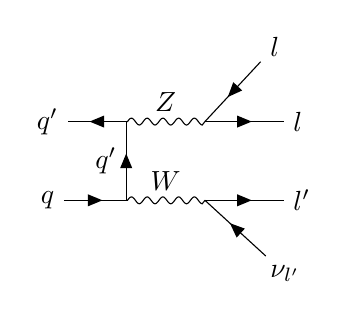
\begin{tikzpicture}
\begin{feynman} [small]
	\vertex (a1) {\(q'\)};
	\vertex [below=of a1] (a2) {\(q\)};
	
	\vertex [right=of a1] (b1);
	\vertex [right=of a2] (b2);

	\vertex [right=of b1] (c1);
	\vertex [right=of b2] (c2);

 	\vertex [above right=of c1] (l1) {\(l\)};
 	\vertex [right=of c1] (l2) {\(l\)};
 	
 	\vertex [right=of c2] (l3) {\(l'\)};
 	\vertex [below right=of c2] (v1) {\(\nu_{l'}\)};

    \diagram* {

    (a2) -- [fermion] (b2),
    (b2) -- [fermion, edge label=\(q'\)] (b1),
    (b1) -- [fermion] (a1), 
	
	(b1) -- [boson, edge label=\(Z\)] (c1),
	(b2) -- [boson, edge label=\(W\)] (c2),

	(l1) -- [fermion] (c1) -- [fermion] (l2),
	(v1) -- [fermion] (c2) -- [fermion] (l3),

    };

\end{feynman}
\end{tikzpicture}

\end{document}
